\documentclass[tikz,border=0pt]{standalone}
\usepackage[T1]{fontenc}
\usepackage[scaled=0.94]{helvet}
\renewcommand{\familydefault}{\sfdefault}
\usepackage{amsmath}
\usepackage{xcolor}
\usetikzlibrary{arrows.meta,calc,patterns}

\definecolor{OIblue}{HTML}{0072B2}
\definecolor{OIorange}{HTML}{E69F00}
\definecolor{OIgreen}{HTML}{009E73}
\definecolor{OIred}{HTML}{D55E00}
\definecolor{OIpurple}{HTML}{CC79A7}
\definecolor{OIsky}{HTML}{56B4E9}
\definecolor{OIdark}{HTML}{343A40}

\tikzset{
  every node/.style={font=\fontsize{7.2}{8.3}\selectfont},
  panel/.style={draw=gray!55,fill=gray!2,rounded corners=2pt,line width=.55pt},
  sourcebox/.style={draw=gray!55,fill=white,rounded corners=1.2pt,line width=.45pt},
  block/.style={draw=gray!60,fill=white,rounded corners=1.3pt,line width=.5pt,inner sep=2pt,align=center},
  flow/.style={-{Latex[length=1.35mm,width=1mm]},draw=OIdark!82,line width=.65pt},
  queryflow/.style={-{Latex[length=1.35mm,width=1mm]},draw=OIpurple!90!black,line width=.7pt},
  poscell/.style={draw=gray!55,fill=OIblue,line width=.35pt},
  negcell/.style={draw=gray!55,fill=white,line width=.35pt},
  unknowncell/.style={draw=gray!60,fill=gray!10,pattern=north east lines,pattern color=gray!65,line width=.35pt}
}

\newcommand{\drawdata}[3]{%
  \ifnum#3=2
    \path[unknowncell] (#1,#2) rectangle ++(.50,.22);
    \node[font=\fontsize{7}{8}\selectfont] at ($ (#1,#2)+(0.25,0.11) $) {?};
  \else
    \ifnum#3=1
      \path[poscell] (#1,#2) rectangle ++(.50,.22);
      \node[font=\fontsize{7}{8}\selectfont,text=white] at ($ (#1,#2)+(0.25,0.11) $) {1};
    \else
      \path[negcell] (#1,#2) rectangle ++(.50,.22);
      \node[font=\fontsize{7}{8}\selectfont,text=gray!65] at ($ (#1,#2)+(0.25,0.11) $) {0};
    \fi
  \fi
}

\newcommand{\sourceblock}[3]{%
  \coordinate (sbase) at (.27,#1);
  \draw[sourcebox] (sbase) rectangle ($(sbase)+(3.72,1.48)$);
  \node[anchor=west,font=\bfseries\fontsize{7.4}{8.4}\selectfont] at ($(sbase)+(.12,1.29)$) {#2};
  \foreach \col/\head in {0/AF,1/RBBB,2/IHD,3/SB} {
    \pgfmathsetmacro{\hx}{1.17+.62*\col}
    \node[font=\fontsize{7}{8}\selectfont] at ($(sbase)+(\hx,1.03)$) {\head};
  }
  \foreach \r/\a/\b/\c/\d in {#3} {
    \pgfmathsetmacro{\yy}{.22+(3-\r)*.25}
    \pgfmathsetmacro{\yc}{\yy+.11}
    \pgfmathsetmacro{\absY}{#1+\yy}
    \node[anchor=east,font=\fontsize{7}{8}\selectfont] at ($(sbase)+(.83,\yc)$) {R\r};
    \pgfmathsetmacro{\xone}{.27+.92}
    \pgfmathsetmacro{\xtwo}{.27+1.54}
    \pgfmathsetmacro{\xthree}{.27+2.16}
    \pgfmathsetmacro{\xfour}{.27+2.78}
    \drawdata{\xone}{\absY}{\a}
    \drawdata{\xtwo}{\absY}{\b}
    \drawdata{\xthree}{\absY}{\c}
    \drawdata{\xfour}{\absY}{\d}
  }
}

\begin{document}
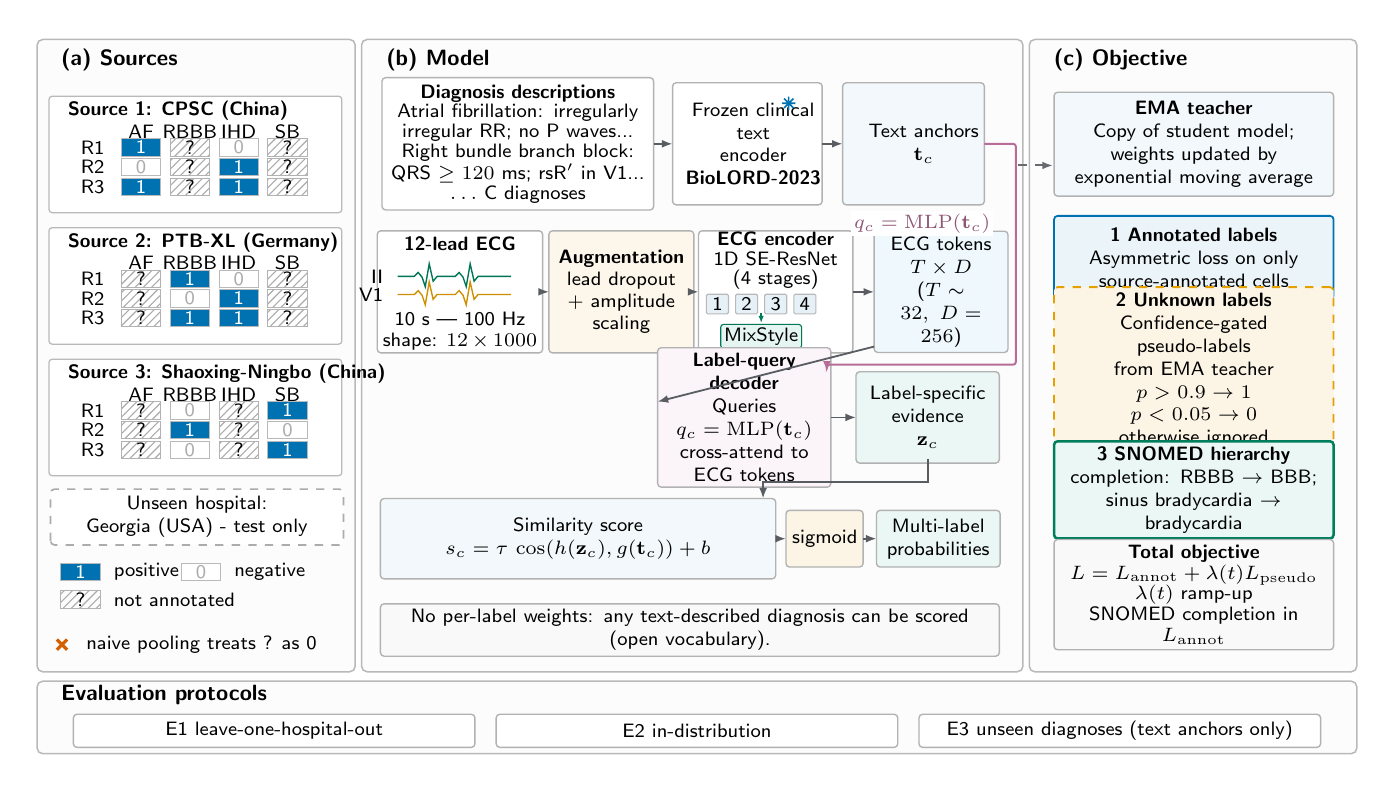
\begin{tikzpicture}[x=1cm,y=1cm]
  \path[use as bounding box] (0,0) rectangle (17,9.3);

  % Three aligned panels and the full-width evaluation strip
  \draw[panel] (.12,1.12) rectangle (4.16,9.15);
  \draw[panel] (4.24,1.12) rectangle (12.64,9.15);
  \draw[panel] (12.72,1.12) rectangle (16.88,9.15);
  \draw[panel] (.12,.08) rectangle (16.88,1.00);

  \node[anchor=west,font=\bfseries\fontsize{8.5}{9.4}\selectfont] at (.30,8.89) {(a) Sources};
  \node[anchor=west,font=\bfseries\fontsize{8.5}{9.4}\selectfont] at (4.43,8.89) {(b) Model};
  \node[anchor=west,font=\bfseries\fontsize{8.5}{9.4}\selectfont] at (12.91,8.89) {(c) Objective};

  % Panel (a): source-specific annotation masks
  \sourceblock{6.95}{Source 1: CPSC (China)}{1/1/2/0/2,2/0/2/1/2,3/1/2/1/2}
  \sourceblock{5.28}{Source 2: PTB-XL (Germany)}{1/2/1/0/2,2/2/0/1/2,3/2/1/1/2}
  \sourceblock{3.61}{Source 3: Shaoxing-Ningbo (China)}{1/2/0/2/1,2/2/1/2/0,3/2/0/2/1}

  \draw[draw=gray!65,dashed,rounded corners=1.5pt,line width=.6pt,fill=white]
    (.29,2.73) rectangle (4.01,3.44);
  \node[align=center,text width=3.45cm,font=\fontsize{7.2}{8.3}\selectfont]
    at (2.15,3.085) {Unseen hospital:\\Georgia (USA) - test only};

  % Annotation legend
  \drawdata{.42}{2.28}{1}
  \node[anchor=west] at (.97,2.39) {positive};
  \drawdata{1.95}{2.28}{0}
  \node[anchor=west] at (2.50,2.39) {negative};
  \drawdata{.42}{1.93}{2}
  \node[anchor=west] at (.97,2.04) {not annotated};

  \draw[OIred,line width=1.15pt] (.37,1.40)--(.50,1.53);
  \draw[OIred,line width=1.15pt] (.37,1.53)--(.50,1.40);
  \node[anchor=west] at (.62,1.465) {naive pooling treats ? as 0};

  % Panel (b): text branch
  \node[block,minimum width=3.45cm,minimum height=1.68cm,text width=3.25cm]
    at (6.225,7.825)
    {\parbox{3.25cm}{\centering\fontsize{7}{7.1}\selectfont
      \textbf{Diagnosis descriptions}\\
      Atrial fibrillation: irregularly irregular RR; no P waves...\\
      Right bundle branch block: QRS $\geq 120$ ms; rsR$'$ in V1...\\
      $\ldots$ C diagnoses}};
  \node[block,minimum width=1.90cm,minimum height=1.55cm,text width=1.70cm]
    at (9.14,7.825)
    {\parbox{1.85cm}{\centering\fontsize{7.2}{8.2}\selectfont
      Frozen clinical text\\encoder\\\textbf{BioLORD-2023}}};
  \node[block,minimum width=1.80cm,minimum height=1.55cm,text width=1.60cm,fill=OIblue!5]
    at (11.25,7.825)
    {\parbox{1.86cm}{\centering\fontsize{7.2}{8.2}\selectfont
      Text anchors\\$\mathbf{t}_c$}};
  \draw[flow] (7.95,7.825)--(8.19,7.825);
  \draw[flow] (10.09,7.825)--(10.35,7.825);

  % Snowflake marker for the frozen encoder
  \draw[OIblue,line width=.55pt]
    (9.58,8.34)--(9.75,8.34)
    (9.665,8.255)--(9.665,8.425)
    (9.605,8.28)--(9.725,8.40)
    (9.605,8.40)--(9.725,8.28);

  % ECG input, augmentation, encoder and tokens
  \node[block,minimum width=2.10cm,minimum height=1.55cm,text width=1.96cm]
    at (5.49,5.945) {};
  \node[font=\bfseries\fontsize{7.2}{8.3}\selectfont] at (5.49,6.56) {12-lead ECG};
  \begin{scope}[xshift=-4pt,yshift=4pt]
  \node[anchor=east,font=\fontsize{7}{8}\selectfont] at (4.78,6.00) {II};
  \node[anchor=east,font=\fontsize{7}{8}\selectfont] at (4.78,5.77) {V1};
  \draw[OIgreen!75!black,line width=.5pt]
    (4.84,6.00)--(5.05,6.00)--(5.10,6.05)--(5.15,5.99)--(5.19,5.87)--(5.24,6.16)--(5.29,5.94)--(5.34,6.00)--(5.57,6.00)--(5.62,6.05)--(5.67,5.99)--(5.71,5.87)--(5.76,6.16)--(5.81,5.94)--(5.86,6.00)--(6.28,6.00);
  \draw[OIorange!90!black,line width=.5pt]
    (4.84,5.77)--(5.05,5.77)--(5.10,5.82)--(5.15,5.76)--(5.19,5.64)--(5.24,5.93)--(5.29,5.71)--(5.34,5.77)--(5.57,5.77)--(5.62,5.82)--(5.67,5.76)--(5.71,5.64)--(5.76,5.93)--(5.81,5.71)--(5.86,5.77)--(6.28,5.77);
  \end{scope}  \node[font=\fontsize{7}{8}\selectfont] at (5.49,5.445) {\parbox{1.96cm}{\centering\fontsize{7}{7.5}\selectfont 10 s | 100 Hz\\shape: $12\times1000$}};

  \node[block,minimum width=1.84cm,minimum height=1.55cm,text width=1.70cm,fill=OIorange!8]
    at (7.54,5.945)
    {\parbox{1.70cm}{\centering\fontsize{7}{8}\selectfont
      \textbf{Augmentation}\\lead dropout\\+ amplitude\\scaling}};
  \node[block,minimum width=1.96cm,minimum height=1.55cm,text width=1.80cm]
    at (9.50,5.945) {};
  \node at (9.50,6.34)
    {\parbox{1.80cm}{\centering\fontsize{7}{7}\selectfont
      \textbf{ECG encoder}\\1D SE-ResNet\\(4 stages)}};
  \foreach \sx/\lab in {8.76/1,9.13/2,9.50/3,9.87/4} {
    \node[draw=gray!55,fill=OIblue!10,rounded corners=.5pt,minimum width=.28cm,minimum height=.25cm,inner sep=0pt]
      at (\sx,5.79) {\lab};
  }
  \draw[OIgreen!80!black,-{Latex[length=.9mm,width=.7mm]},line width=.55pt]
    (9.315,5.68)--(9.315,5.55);
  \node[draw=OIgreen!75!black,fill=OIgreen!10,rounded corners=1pt,inner sep=1.2pt,
        font=\fontsize{7}{8}\selectfont]
    at (9.315,5.38) {MixStyle};

  \node[block,minimum width=1.70cm,minimum height=1.25cm,text width=1.52cm,fill=OIsky!10]
    at (11.60,5.945)
    {\parbox{1.52cm}{\centering\fontsize{7.2}{8.3}\selectfont
      ECG tokens\\$T\times D$\\($T\sim32,\ D=256$)}};

  \draw[flow] (6.54,5.945)--(6.62,5.945);
  \draw[flow] (8.46,5.945)--(8.52,5.945);
  \draw[flow] (10.48,5.945)--(10.75,5.945);

  % Label queries and cross-attention
  \node[block,minimum width=2.20cm,minimum height=1.16cm,text width=2.02cm,fill=OIpurple!8]
    at (9.10,4.35)
    {\parbox{2.02cm}{\centering\fontsize{7.2}{8.3}\selectfont
      \textbf{Label-query decoder}\\
      Queries $q_c=\mathrm{MLP}(\mathbf{t}_c)$\\cross-attend to ECG tokens}};
  \node[block,minimum width=1.82cm,minimum height=1.16cm,text width=1.62cm,fill=OIgreen!8]
    at (11.43,4.35)
    {\parbox{1.62cm}{\centering\fontsize{7.2}{8.3}\selectfont
      Label-specific evidence\\$\mathbf{z}_c$}};
  \draw[flow] (10.75,5.25)--(8.00,4.55);
  \draw[flow] (10.20,4.35)--(10.52,4.35);
  \node[font=\fontsize{7}{8}\selectfont,text=OIpurple!70!black,fill=white,inner sep=1pt]
    at (11.36,6.81) {$q_c=\mathrm{MLP}(\mathbf{t}_c)$};
  \draw[queryflow,rounded corners=1pt]
    (12.15,7.825)--(12.55,7.825)--(12.55,5.02)--(10.15,5.02)--(10.15,4.93);

  % Similarity scoring, probabilities and open-vocabulary note
  \node[block,minimum width=5.02cm,minimum height=1.02cm,text width=4.82cm,fill=OIblue!5]
    at (6.99,2.81)
    {\parbox{4.82cm}{\centering\fontsize{7.2}{8.3}\selectfont
      Similarity score\\
      $s_c=\tau\,\cos\!\left(h(\mathbf{z}_c),g(\mathbf{t}_c)\right)+b$}};
  \node[block,minimum width=.98cm,minimum height=.72cm,text width=.82cm,fill=OIorange!10]
    at (10.12,2.81) {\fontsize{7}{8}\selectfont sigmoid};
  \node[block,minimum width=1.57cm,minimum height=.72cm,text width=1.38cm,fill=OIgreen!8]
    at (11.565,2.81)
    {\parbox{1.38cm}{\centering\fontsize{7.2}{8.3}\selectfont Multi-label\\probabilities}};
  \draw[flow] (9.50,2.81)--(9.63,2.81);
  \draw[flow] (10.61,2.81)--(10.78,2.81);
  \draw[flow] (11.43,3.825)--(11.43,3.53)--(9.34,3.53)--(9.34,3.32);
  \node[block,minimum width=7.86cm,minimum height=.66cm,text width=7.66cm,fill=gray!5]
    at (8.41,1.65)
    {\parbox{7.66cm}{\centering\fontsize{7.2}{8.3}\selectfont
      No per-label weights: any text-described diagnosis can be scored (open vocabulary).}};

  % Panel (c): EMA teacher and annotation-aware objective components
  \node[block,minimum width=3.55cm,minimum height=1.32cm,text width=3.28cm,fill=OIblue!5]
    at (14.81,7.82)
    {\parbox{3.28cm}{\centering\fontsize{7.2}{8.3}\selectfont
      \textbf{EMA teacher}\\
      Copy of student model; weights updated by exponential moving average}};
  \draw[-{Latex[length=1.35mm,width=1mm]},draw=OIdark!75,dashed,line width=.7pt]
    (12.58,7.55)--(13.02,7.55);

  \node[draw=OIblue,fill=OIblue!8,rounded corners=1.3pt,line width=.65pt,
        minimum width=3.55cm,minimum height=1.06cm,text width=3.26cm,inner sep=2pt,align=center]
    at (14.81,6.38)
    {\parbox{3.26cm}{\centering\fontsize{7.2}{8.3}\selectfont
      \textbf{1  Annotated labels}\\
      Asymmetric loss on only source-annotated cells}};
  \node[draw=OIorange,dashed,fill=OIorange!10,rounded corners=1.3pt,line width=.65pt,
        minimum width=3.55cm,minimum height=1.65cm,text width=3.26cm,inner sep=2pt,align=center]
    at (14.81,4.95)
    {\parbox{3.26cm}{\centering\fontsize{7.2}{8.3}\selectfont
      \textbf{2  Unknown labels}\\
      Confidence-gated pseudo-labels\\
      from EMA teacher\\
      $p>0.9\to1$\\
      $p<0.05\to0$\\
      otherwise ignored}};
  \node[draw=OIgreen!80!black,fill=OIgreen!8,rounded corners=1.3pt,line width=.9pt,
        minimum width=3.55cm,minimum height=1.22cm,text width=3.26cm,inner sep=2pt,align=center]
    at (14.81,3.43)
    {\parbox{3.26cm}{\centering\fontsize{7.2}{8.3}\selectfont
      \textbf{3  SNOMED hierarchy}\\
      completion: RBBB $\to$ BBB;\\
      sinus bradycardia $\to$ bradycardia}};
  \node[block,minimum width=3.55cm,minimum height=1.26cm,text width=3.28cm,fill=gray!5]
    at (14.81,2.10)
    {\parbox{3.28cm}{\centering\fontsize{7}{7.5}\selectfont
      \textbf{Total objective}\\
      $L=L_{\mathrm{annot}}+\lambda(t)L_{\mathrm{pseudo}}$\\
      $\lambda(t)$ ramp-up\\
      SNOMED completion in $L_{\mathrm{annot}}$}};

  % Bottom evaluation protocols
  \node[anchor=west,font=\bfseries\fontsize{7.6}{8.5}\selectfont] at (.30,.82) {Evaluation protocols};
  \node[block,minimum width=5.10cm,minimum height=.42cm,text width=4.88cm,fill=white]
    at (3.13,.37) {E1  leave-one-hospital-out};
  \node[block,minimum width=5.10cm,minimum height=.42cm,text width=4.88cm,fill=white]
    at (8.50,.37) {E2  in-distribution};
  \node[block,minimum width=5.10cm,minimum height=.42cm,text width=4.88cm,fill=white]
    at (13.87,.37) {E3  unseen diagnoses (text anchors only)};
\end{tikzpicture}
\end{document}
